\chapter{Introduction}
\label{chapter:introduction}

One of the main goals in computer graphics is realistic rendering. 
Even though computer graphics is constantly improving, we are still quite away from reality because material representation in a traditional way lack important realistic properties. 
A 2-D texture in conjunction with a shading model is a conventional way to represent material appearances in rendering.
Real-world materials surfaces on the other hand consist of surface meso-structures, i.e. intermediate in between micro and macro structures.
Meso-structures are responsible for fine-scale shadows, self-occlusions, inter-reflection, subsurface scattering and specularities.
Also, reflectance and the look of real-world materials can drastically change when camera and light directions vary.

One of the possible solution to represent such material attributes is to use sophisticated light functions, for instance a Bidirectional Texture Function (BTF). 
 A BTF is a 6-dimensional function that depends on camera and light directions as well as on spatial texture coordinates. 
The BTF conceptually extends traditional 2-D textures by the dependence on light and camera directions.
This function is usually acquired as a data-set of thousands of images that cover discrete light and camera directions.
Due to the enormous size of that data direct renderings even on modern hardware without any compression is impractical.
Fortunately, many techniques exist to deal with the huge size of BTFs, i.e. compression methods.


In this thesis, we use \emph{WebGL} for real-time rendering of BTF in the Web.
Even though 3-D graphics for the Web becoming more and more popular. BTFs are rarely used realistic rendering, due to their huge size and the overall computational effort needed for rendering,
including decompression of the data and interpolation of camera and light directions.
Such demanding computational effort is time consuming, especially for on mobile-devices.

And the problem which arises when rendering BTFs in a Browser is the transmission of the data.
Before rendering on the client side, the transmission of the data has to be finished.
Even the transfer of a compressed BTF data can take a considerable amount of time. 
The compressed BTF can be tens of megabytes in size.
Because users are eager to see a result, especially on the Web, we use a streaming solution to deliver the data as quickly as possibly, while steadily increasing the resulting image.
 \emph{Web-Sockets} are the state of the art technique for streaming and are supported by most of today's browsers.
With \emph{Web-Sockets}  a  full-duplex communication is available for the server and the client, which is faster than traditional HTTP-based methods. 
This promises fast and reliable solution for real-time performance in \emph{WebGL}-based application.

In this thesis we use a PCA for compression, which allows for a considerably good compression ratio with low decompression error.
Also, it is well suited for real-time rendering and streaming.

We implemented WebGL demo web-application and \emph{Web-Sockets} server for streaming purposes.



\section{Related Work}
\label{section:related_work}

Nowadays, Web technologies are able to support WebGL \cite{webgl}, which is a JavaScript API for rendering 3D content.
WebGL provides  vertex and fragment shaders  for creating highly realistic rendering results.
New standards for 3D graphics in context of HTML domain are evolving, for instance such as XML3D \cite{xml3d}.
XML3D allows for embedding 3D graphics into HTML pages. XML3D is based both on XML and WebGL.
It allows for declaring 3D scenes elements in the context of HTML pages.
Web programmers can apply their existing knowledge (i.e. about DOM, XML, CSS) to include 3D graphics in the HTML content by using XML3D.
Currently XML3D  natively supported by  Firefox and Google Chrome browsers on Linux and Windows.
 
Most of previous work that used BTFs for realistic rendering were primarily intended  for offline applications.
However, their approach is not suitable in the context of the Web, due to the data transfer between the server and a client.
  Schwartz \emph{et. al.} \cite{webglbtfstreaming} presented a work in which compressed BTF data is streamed from the server to a client.
 The streaming over the Internet is done by means of HTTP streaming, i.e. the web-application requests the data in small chunks.
 With each new chunk of the BTF data the rendering quality of the 3D object is progressively enhanced.
 We on the other hand, use \emph{Web-Sockets} to improve application performance compared to HTPP streaming, by reducing the network latency and streaming the data in a binary form.

 
Existing BTF compression methods are reviewed by Haindl \emph{et. al.} \cite{haindl, haindl_visual}.
A trade-off has to be made between the rendering quality and compression rate depending on the intended application.
 Our compression method is related to the PCA RF (Principal Component Analysis Reflectance Field) method, which was introduced by Sattler \emph{et. al.} \cite{star2004}.
This method allows for real-time performance with realistic rendering quality. 
Sattler performs PCA on each of the $n$ camera directions separately. We on the other hand, perform PCA on $k$ neighbour camera directions at once.
In Haindl's review \cite{haindl} PCA based methods achieve better or at least equal reconstruction results than most other methods.
Compression rates of PCA methods are not as high as those of other methods. However, those methods, which produce better compression rates, have worse quality than PCA based methods.



\section{Outline}
\label{section:outline}

\begin{figure}[h]
 \centering
 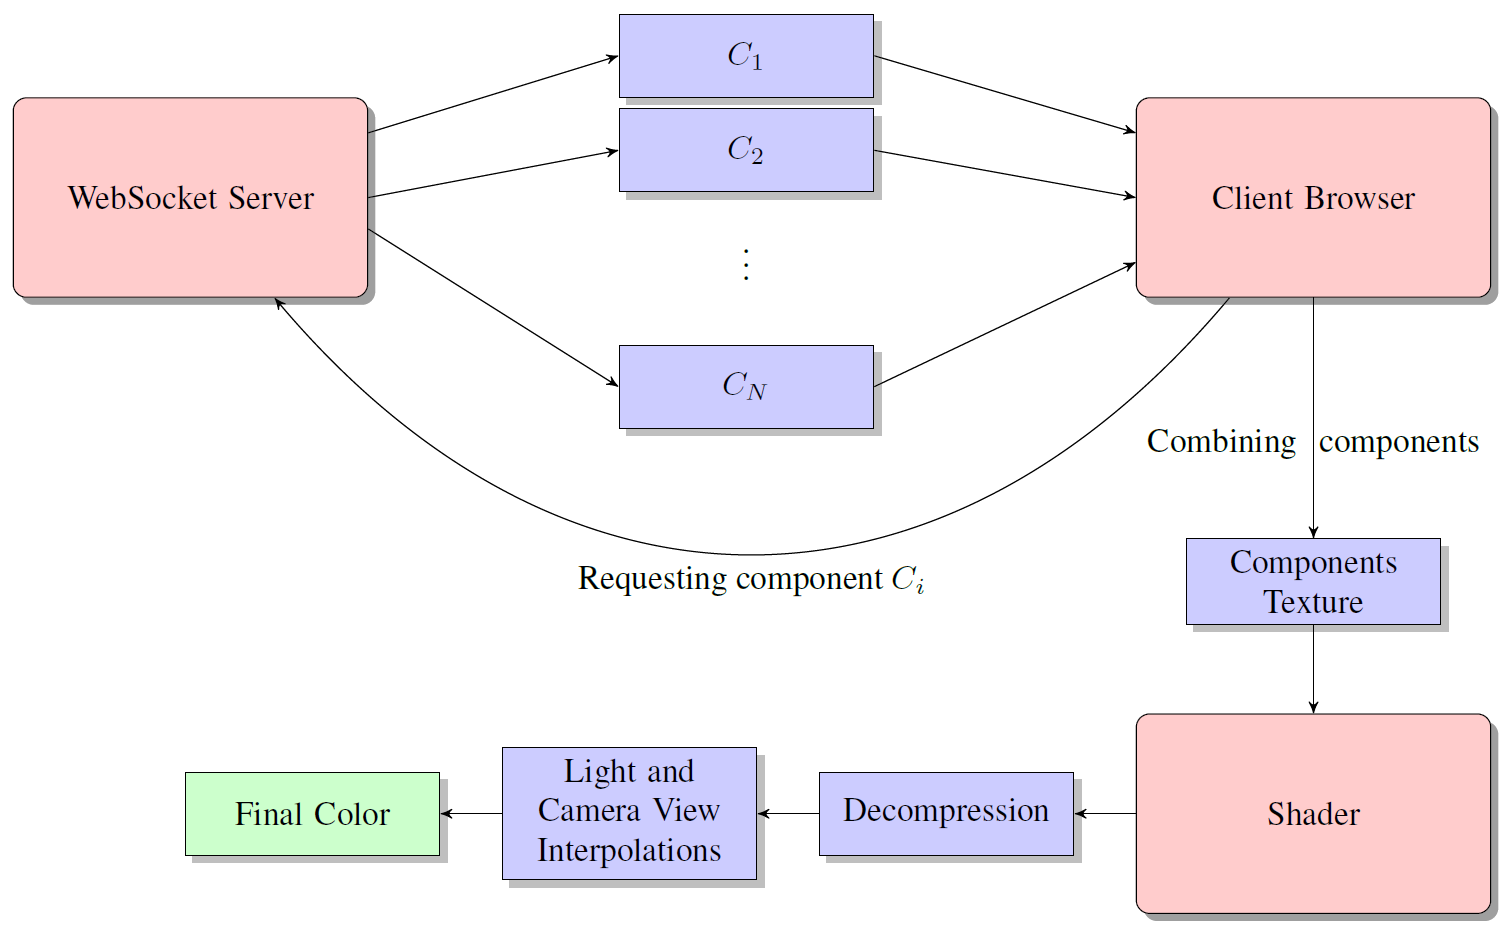
\includegraphics[width=1.0\textwidth]{figures/overview}
 \caption[Model Overview ] {
 	{\bf Model Overview}

	
	}
 \label{fig:overview}
\end{figure}



